% \documentclass{report}
\documentclass[12pt]{report}
%\documentclass[a4paper,12pt]{report}

% IMPORT PACKAGE
\usepackage{lmodern}
\usepackage{hyperref}
\usepackage[T1]{fontenc}
\usepackage{geometry} 
\usepackage{graphicx}
\usepackage[french]{babel}
\usepackage{tikz}
\usetikzlibrary{calc}
\usepackage{fancyhdr}
\usepackage{titlesec}
\usepackage{listings}
\usetikzlibrary{shapes, arrows}

% PADDING
\geometry{
  a4paper,
  left=20mm,
  right=20mm,
  headheight=2cm,
  top=3cm,
  bottom=5cm,
  footskip=4cm
}

% Insérer une page blanche sans en-tête et sans pied de page
\newcommand\EmptyPage{
    \newpage
    \null
    \thispagestyle{empty}
    \addtocounter{page}{-1}
    \newpage}

\hypersetup{
    colorlinks=true,
    linkcolor=blue,
    filecolor=magenta,
    urlcolor=cyan,
}


% FRONT COVER
\renewcommand{\titlepage}{%
  \begin{tikzpicture}[remember picture,overlay]
    \node[inner sep=0pt] at (current page.center) {\includegraphics[width=\paperwidth,height=\paperheight]{Includes/Images/pageDeGarde2.jpg}};
  \end{tikzpicture}%
}

% HEAD & FOOTER
\pagestyle{fancy}

\fancyhead[L]{
\includegraphics[width=2cm]{Includes/Images/Dept_Marketplaces_Logo.png}}
\fancyhead[C]{Rapport d'activité stage, 4 semaines.}
\fancyhead[R]{
\includegraphics[width=1.5cm]{Includes/Images/universitedecorse.png}}

\fancyfoot[L]{Anthony Menghi}
\fancyfoot[C]{\thepage}
\fancyfoot[R]{\today}

\fancypagestyle{plain}{\pagestyle{fancy}}

% \fancypagestyle{plain}{% Redefine plain style
%     \fancyhf{} % Clear header and footer

%     \fancyhead[R]{
\includegraphics[width=2cm]{Includes/Images/universitedecorse.png}}
  
%     % Includes/Images/universitedecorse.png
%     \fancyhead[C]{Rapport d'activité stage, 4 semaines.}

%     \fancyhead[L]{
\includegraphics[width=2cm]{Includes/Images/Dept_Marketplaces_Logo.png}}
    

%     \fancyfoot[R]{18/05/2024} % Ajout du comptage de page
%     \fancyfoot[C]{\thepage}
%     \fancyfoot[L]{Anthony Menghi}
% }
% % Apply "plain" page style to all pages
% \pagestyle{plain}

% \title{Rapport de Stage - BUT MMI 2 \\ \Large Università di Corsica Pasquale Paoli}
% \author{Anthony Menghi}
% \date{June 2023}
\title{}
\author{}
\date{}

\begin{document}
\thispagestyle{empty} %enelver le page de style sur la page de couverture 
\maketitle 
\EmptyPage
% COVER PAGE
% UNIVERSITY
\vspace*{1cm}

\textbf{\Large Rapport d'activité de stage de 4 semaines}
\vspace*{0.8cm}

\textbf{Création d'une UX/UI dynamique avec Relume et Webflow : Anaylse, rapport et développement React avec Next.js et Headless CMS}
\vspace*{1cm}

\textbf{\underline{\Large Université :}}

\begin{figure}[h]

\includegraphics[width=0.15\textwidth]{Includes/Images/universitedecorse.png} 
\end{figure}

\begin{flushleft}
    \hspace{1cm} Università di Corsica Pasquale Paoli \\
    \hspace{1cm} Faculté des Sciences et techniques.\\
    \hspace{1cm} Campus Grimaldi, BP 52, 20250, Corte, France.\\
\end{flushleft}
\vspace{0.8cm}


% LABORATORY
\textbf{\underline{\Large Entreprise :}}

\begin{figure}[h] 

\includegraphics[width=0.2\textwidth]{Includes/Images/Dept_Marketplaces_Logo.png} 
\end{figure}

\begin{flushleft}
    \hspace{1cm} DEPT® \\
    \hspace{1cm} Full service digital agency - Pioneering tech/marketing \\
    \hspace{1cm} 24 Earlsfort Terrace,\\
    \hspace{1cm} D02 KC42, \\
    \hspace{1cm} Dublin , Ireland \\
\end{flushleft}
\vspace{0.8cm}


% STUDENT
\textbf{\underline{\Large Étudiant :}}
\begin{flushleft}
    \hspace{1cm} Anthony MENGHI, \\
    \hspace{1cm} Filière : Licence 3 Sciences pour l'Ingénieur \\
    \hspace{1cm} Parcours : Informatique, \\
    \hspace{1cm} Promotion : 2023. \\
\end{flushleft}
\vspace{0.8cm}
\textbf{\underline{\Large Maître d'apprentissage :}} 
\begin{flushleft}
    \hspace{1cm} M. Marc Raffali \\
    \hspace{1cm} Email : raffalli.marc.ed@gmail.com\\
\end{flushleft}
\vspace{0.8cm}

\textbf{\underline{\Large Tuteur pédagogique:}}  
\begin{flushleft}
    \hspace{1cm} M. Paul-Antoine Bisgambiglia \\
\end{flushleft}
\vspace{0.8cm}

\textbf{\underline{\Large Perdiode de stage :}}  
\begin{flushleft}
    \hspace{1cm} Du 8 avril au 3 mai 2024. \\
\end{flushleft}

\EmptyPage
\chapter*{Engagement de non plagiat}

Je, soussigné, Menghi Anthony, déclare être pleinement conscient que le plagiat de documents ou d’une partie d’un document publiés sur toutes formes de support, y compris l’internet, constitue une violation des droits d’auteur ainsi qu’une fraude caractérisée.  \\
En conséquence, je m’engage à citer toutes les sources que nous avons utilisées pour écrire ce rapport.
\EmptyPage

% NOTE READER
\chapter*{Note de lecture}


Cher lecteur, \\

Ce rapport contient des termes techniques couramment utilisés dans le domaine de l'informatique, tels que l'API, Headless CMS, etc. Des définitions de ces termes sont fournis via des notes de bas de page tout au long du texte, à partir de l'introduction. \\
Ces ressources vous aideront à mieux appréhender les concepts techniques présentés dans ce rapport. \\ 

Cordialement, \\ 

Anthony Menghi.
\EmptyPage
% ABSTRACTS
\chapter*{Synthèse}

Ce stage s'inscrit au sein de l'entreprise DEPT, au sein du département irlandais. DEPT est une entreprise pionnière en technologie et en marketing qui aide ses clients à garder une longueur d'avance. C'est une agence numérique à service complet, avec une équipe de plus de 4 000 spécialistes du numérique répartis sur plus de 30 sites sur cinq continents. Elle travaille à l'échelle mondiale avec des clients renommés tels qu'Adidas, Patagonia, Google Workspace et bien d'autres. DEPT combine narration créative et technologie pour créer des expériences numériques complètes, optimisant tout le parcours client. De plus, elle conçoit, construit et intègre des logiciels et du matériel pour les principales entreprises SaaS et traditionnelles.

Au cours de ce stage, ma mission a été de tester différents services, mettre en relation des outils, développer des solutions informatiques pour créer une UI et une UX totalement dynamiques. Afin de résoudre plusieurs problèmes comme la répétition du travail, le manque de synergie entre différents métiers tels que les designers graphiques, les content managers et les développeurs.

La solution développée pendant le stage permet de connecter la création de wireframes, le style graphique, le code et le contenu des pages en quelques clics pour permettre une meilleure expérience de travail et de relation entre les différents processus de création, afin de gagner en efficacité.

Ce stage m'a permis de découvrir le travail dans une entreprise internationale, l'ingénierie, la mise en place de projets, notamment en termes de gestion de projet, de processus d'automatisation et de différentes méthodes de travail. J'ai également eu l'opportunité de découvrir différents outils et services à la pointe de la technologie. J'ai également pu renforcer mes compétences en développement web en testant et en développant avec JavaScript, React et Next.js. Enfin, j'ai appris de nouvelles façons de coder avec l'apprentissage de nouveaux motifs d'architecture logicielle, de nouveaux outils et une nouvelle approche de l'utilisation de l'intelligence artificielle.

Grâce à ce stage, j'ai pu participer à un projet concret qui m'a permis de découvrir la mise en place et la réflexion de projets dans une entreprise internationale.
\\ \\
\textbf{Mots-clés :} Processus d'automatisation, Développement web, JavaScript, React, Next.js, Headless CMS, Service d'intelligence artificielle, Méthodes de travail, Motifs d'architecture logicielle, Gestion de projet.

\EmptyPage
% \include{Includes/Abstracts/abstract}
% \EmptyPage
% \include{Includes/Abstracts/riassuntu}
% \EmptyPage
% ACKNOWLEDGEMENTS
% \chapter*{Remmerciements}

Je tiens tout d'abord à exprimer ma profonde gratitude envers les personnes qui ont contribué à la réussite de mon stage et à mon enrichissement personnel. Je souhaite adresser mes sincères remerciements à :

\begin{itemize}

\item M. Marc Raffalli, mon tuteur de stage, pour m'avoir accordé sa confiance et de m'avoir offert une partie de son temps pour me guider et m'accompagner tout au long de mon stage. Son expertise, ses conseils avisés et sa bienveillance ont été des atouts précieux dans la réalisation de ce projet.

\item L'équipe pédagogique de la Licence 3 SPI parcours Informatique. Je souhaite exprimer ma gratitude envers les enseignants et les membres du personnel administratif qui ont contribué à ma formation et qui ont toujours été présents pour répondre à mes questions et me guider dans mon parcours.

\item L'Université de Corse pour avoir mis à ma disposition les infrastructures nécessaires à la réalisation de mon stage. Leur soutien logistique et administratif a grandement facilité le bon déroulement de cette expérience professionnelle.
\end{itemize}

Enfin, je tiens à remercier tous ceux qui, de près ou de loin, ont contribué à la réussite de mon stage, notamment mes collègues de travail qui ont partagé leurs connaissances et leur expérience avec générosité. Leur implication et leur soutien ont été des facteurs déterminants dans l'enrichissement de mes compétences et dans la réussite de ce stage.

Je leur suis profondément reconnaissant et je garde un souvenir précieux de cette expérience.
% \EmptyPage
% TABLES OF COTENT
\tableofcontents
\EmptyPage
% INTRODUCTION
\chapter{Introduction}
Ce rapport de stage retrace mon expérience au sein de l'entreprise DEPT, dans son département irlandais. DEPT est une entreprise innovante dans les domaines de la technologie et du marketing, permettant à ses clients de toujours rester en avance. En tant qu'agence numérique proposant une gamme complète de services, DEPT réunit plus de 4 000 experts en numérique, répartis sur plus de 30 sites à travers cinq continents. Collaborant à l'échelle mondiale avec des clients prestigieux comme Adidas, Patagonia, Google Workspace, et bien d'autres, DEPT marie la narration créative à la technologie pour offrir des expériences numériques globales, optimisant ainsi chaque étape du parcours client. En outre, l'entreprise conçoit, développe et intègre des logiciels et du matériel pour les principales sociétés SaaS et traditionnelles.

Dans le cadre de mon stage, ma mission consistait à tester divers services, interconnecter des outils et développer des solutions informatiques visant à créer une interface utilisateur (UI) et une expérience utilisateur (UX) entièrement dynamiques. L'objectif était de résoudre plusieurs problématiques, notamment la répétition des tâches et le manque de synergie entre différents métiers comme les designers graphiques, les content managers et les développeurs.

Le présent rapport se concentre plus particulièrement sur ma contribution au développement d'une solution innovante permettant de relier différents outils pour intégrer la création de wireframes, le style graphique, le code et le contenu des pages en seulement quelques clics. Cela visait à améliorer l'expérience de travail et la collaboration entre les différents processus créatifs, afin d'accroître l'efficacité.
\\ \\
La première partie de ce rapport présente le contexte général du projet. J'y expose mes motivations personnelles qui m'ont conduit à m'engager dans ce stage, ainsi que les objectifs et les projets de l'entreprise DEPT. Je détaille également le cahier des charges, la gestion du temps pendant le stage et la gestion des projets au sein de l'entreprise.


La deuxième partie constitue le cœur de mon travail durant ce stage. J'y décris l'intégration des différents outils en suivant plusieurs étapes. Tout d'abord, je présente ces outils en détail, en soulignant leurs fonctionnalités et leur utilité. Ensuite, j'expose les réflexions sur les diverses possibilités d'interactions entre ces outils, en expliquant les choix technologiques et les stratégies adoptées.

La troisième partie se concentre sur la logique de développement avec un Headless CMS, développée en collaboration avec l'équipe du projet. J'y détaille le processus de réflexion, les décisions prises et les raisons derrière ces choix.


Enfin, je termine par une analyse critique de la solution développée, en présentant ses avantages et ses inconvénients. Cette évaluation permet de mettre en lumière les points forts du projet tout en identifiant les axes d'amélioration possibles pour l'avenir.
\\ \\
Je conclurai ce rapport en mettant en évidence les compétences que j'ai développées tout au long de mon stage, notamment en matière de développement web, de gestion de projet et de résolution de problèmes. Je soulignerai l'importance du travail d'équipe etl'exploration de nouvelles technologie. Ce rapport permettra ainsi de mieux appréhender les différentes étapes de mon travail, les solutions techniques que nous avons apportées

\EmptyPage
% CONTEXT
% CONTEXT
\chapter{Contexte et cahier des charges}


% PERSONAL PERSPECTIVES
\section{Perspectives personnelles}
Cette expérience professionnelle s'inscrit dans le cadre de mon stage de fin d'année en Licence 3 Sciences pour l'Ingénieur, parcours Informatique, à la Faculté des Sciences et Techniques de l'Université de Corse. J'ai été accueilli par l'entreprise DEPT, au sein de son département en Irlande.

J'ai choisi ce stage afin d'approfondir mes connaissances dans le domaine du web, de découvrir le monde de l'entreprise et de comprendre les méthodes de travail dans un contexte international. Cette opportunité de travailler dans une entreprise située hors de France m'a permis de découvrir de nouvelles pratiques professionnelles. Je suis très honoré de pouvoir apporter, à mon modeste niveau, une contribution à une entreprise de portée mondiale.


% PRESENTATION UNIV & PROJECT
\section{Présentation de DEPT et ses projets}
\subsection{Présentation}
DEPT a été créer en 2005 à Amsterdam au Pays-Bas c'est une entreprise innovante dans les domaines de la technologie et du marketing, aidant ses clients à rester à la pointe. En tant qu'agence numérique complète, DEPT réunit plus de 4 000 experts répartis sur plus de 30 sites à travers cinq continents. Travaillant avec des clients prestigieux tels qu'Adidas, Patagonia, Google Workspace, et bien d'autres, DEPT combine créativité et technologie pour offrir des expériences numériques globales, optimisant chaque étape du parcours client. De plus, l'entreprise conçoit, développe et intègre des solutions logicielles et matérielles pour les principales sociétés SaaS et traditionnelles.

\subsection{Projets de l'entreprise}
Du commerce électronique et des technologies émergentes aux expériences client et à l'architecture cloud, Dept imaginne et met en œuvre des solutions techniques d'avenir qui établissent de nouvelles normes pour les entreprises numériques.
\\ \\
DEPT a réalisé de nombreux projets en voici des exemples.


\subsubsection{Arizona State University}

DEPT collabore avec l'Arizona State University (ASU) pour rendre l'éducation plus accessible et équitable à travers le développement de plateformes éducatives adaptées aux besoins spécifiques des apprenants du monde entier. Depuis plus de six ans, DEPT et ASU ont créé diverses solutions EdTech, notamment:

\begin{itemize}
    \item \textbf{Baobab}: Application pour le réseautage et le mentorat des jeunes leaders africains.
    \item \textbf{me3®}: Outil interactif de planification de carrière basé sur un modèle SaaS.
    \item \textbf{Young Thinkers}: Programme en ligne de préparation à l’université et à la carrière pour les jeunes émiratis et arabes.
    \item \textbf{Intelligent Tutor}: Tuteur intelligent pour l'apprentissage autonome en mathématiques.
\end{itemize}

En utilisant une approche centrée sur l'utilisateur, DEPT garantit que chaque solution est adaptée aux contraintes techniques et culturelles des apprenants, contribuant ainsi à démocratiser l'éducation et à atteindre plus d'un million d'utilisateurs à travers le monde.

\subsubsection{Fingerspelling}

HELLO MONDAY/DEPT® et l'American Society for Deaf Children ont créé \textbf{Fingerspelling.xyz}, une application web utilisant l'apprentissage automatique pour enseigner l'alphabet de la langue des signes américaine (ASL).

Fingerspelling.xyz utilise \textit{MediaPipe Hands} pour suivre les mouvements des mains via une webcam. Un modèle 3D montre comment positionner les mains pour chaque lettre, avec des retours en temps réel.

L'application a enregistré des millions de signes corrects et est utilisée par l'American Society for Deaf Children. Récompenses :
\begin{itemize}
    \item \textbf{Webby Awards 2023}: trois People's Voice Awards. 
    \item \textbf{Webby Awards 2022}: deux Webby Awards et trois People's Voice Awards.
    \item \textbf{Eurobest Awards}: Prix de l'innovation, Or en design.
    \item \textbf{Awwwards}: Site du jour.
    \item \textbf{FWA}: Site du jour et du mois.
    \item \textbf{Cannes Lions}: Or et Argent en design.
    \item \textbf{New York Design Awards 2021}: Argent.
    \item \textbf{Anthem Awards}: Or en Éducation.
\end{itemize}

Fingerspelling.xyz améliore la communication et l'inclusion pour la communauté des Sourds.

\subsection{Participation à l'entreprise}

Dept à de nombreux clients dans l'ecommerce et cherche à concevoir des solutions pour automatiser, éviter de la répétition de taches et améliorer la cohésion entre les différents professionnelles dans le processus de développement et de création
\\ \\
L’équipe qui s’occupe du développement de cet solution est composé de trois personnes : 
\begin{itemize}
    \item M. Derek Brady est le directeur créatif et associé chez DEPT, il s'occupe sur la vision à long terme de l'entreprise, il supervise et à dirige la création et le développement des aspects visuels et créatifs des projets.
    \item M. Marc Raffalli est développeur front-end senior, il s'occupe de l'aspects techniques des projets, il s'est occupé de guider et de m'encadrer tout au long du stage
    \item Enfin, Moi-même, stagiaire ayant pour but de créer la solution pour optimier le processus de création avec l'UI et l'UX dynamique.
\end{itemize}

\section{Cahier des charges}
Le but de ce stage est de créer une solution pour automatiser pour la création d'UI et UX dynamique avec React et Next.js pour les futurs clients de l'entreprise, en utilisant des technologies modernes et en respectant les standards de l'entreprise. 
\\ \\
Cette solution doit permettre de gagner du temps, d'éviter les erreurs et de faciliter la communication entre les différents professionnels.

Il m'a été demandé de tester plusieurs outils et services (Relume, Weblow et Devlink) pour voir si ils peuvent répondre se répondres aux problématiques.

Ensuite, il m'a été demandé d'étudier les différentes possiblité d'interactions entre les outils. 

Puis, de créer un prototype de la solution en utilisant les technologies React et Next.js connecté a un Headless CMS.

Enfin, de tester la solution, de identifié les forces et les faiblesses pour présenter la solution à l'équipe.

% Gestion du temps
\section{Gestion du temps}

Pendant mon stage, j'ai accordé une grande importance à une gestion efficace du temps, afin de maximiser ma productivité et de mener à bien les différentes tâches qui m'ont été confiées. Voici une vue d'ensemble de ma gestion du temps (figure \ref{fig:Diagramme circulaire - Gestion du temps}), basée sur les pourcentages suivants :

\begin{itemize}
\item \textbf{Programmation} : J'ai consacré environ 30\% de mon temps à la programmation. Cela inclut la création le développement en React et Next.js pour créer le prototype de la solution avec la connexion avec le Headless CMS et la mise en place du motif de conception.

\item \textbf{Test des outils} : Environ 25\% de mon temps a été dédié aux tests des outils. J'ai testé les outils Relume, Webflow et Devlink pour voir s'ils répondaient aux besoins du projet et pour identifier les avantages et les inconvénients de chacun.

\item \textbf{Recherche et apprentissage} : Environ 20\% de mon temps a été consacré à la recherche et à l'apprentissage de nouvelles technologies et des nouveaux outils. J'ai appris à utiliser des outils tels que Webflow, Relume et ContentFul pour le headless CMS, et j'ai approfondi mes connaissances en Next.js 14 qui a apporté des changements et nouvelles fonctionnalités.
\item \textbf{Collaboration} : J'ai consacré environ 15\% de mon temps à la collaboration avec l'équipe autour du projet. Cela comprenait des réunions, des discussions et des échanges d'idées pour garantir que le projet prenne la bonne direction, la prise en compte des éventuelles suggestions et la validation de l'avancée de projet.

\item \textbf{Analyse et proposition}: Environ 10\% de mon temps a été consacré à l'analyse des spécifications ; à la proposition de solutions adaptées aux besoins du projet et du cahier des charges. Cette phase m'a permis de comprendre en détail les exigences et d'identifier les meilleures approches pour les satisfaire.
\end{itemize}
\begin{figure}[ht] 
    \centering
    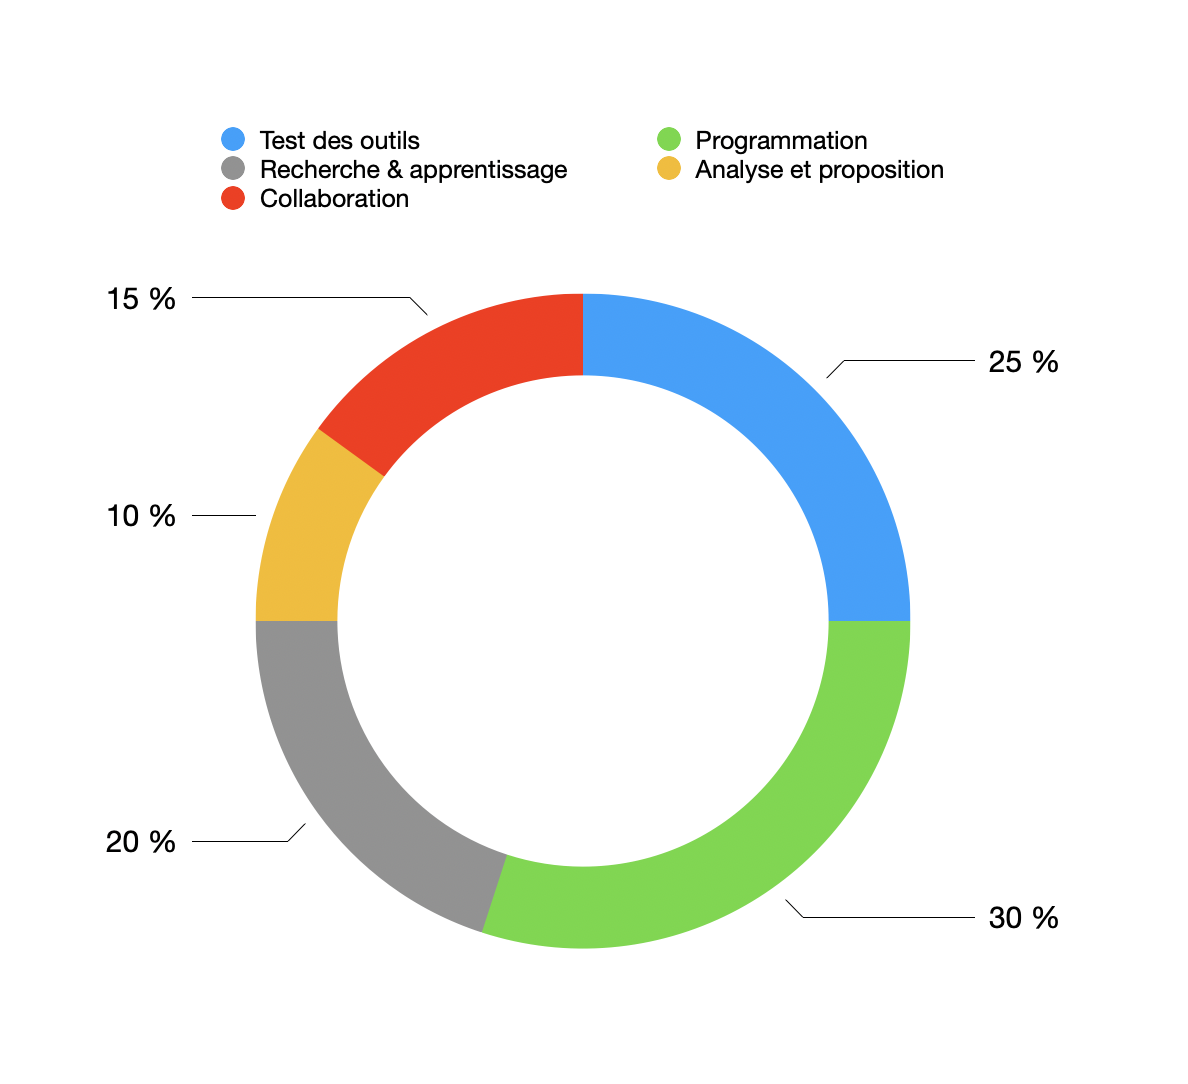
\includegraphics[width=0.7\textwidth]{Includes/Images/gestionTemps.png}
    \caption{Diagramme circulaire - Gestion du temps}
    \label{fig:Diagramme circulaire - Gestion du temps}
\end{figure} 
De ce fait, cette gestion du temps équilibrée m'a permis de mener à bien mes tâches et d'atteindre les objectifs fixés dans les délais impartis. Cette répartition réfléchie du temps m'a permis de rester organisé, de faire face aux défis et d'obtenir des résultats positifs tout au long de mon stage.

\subsection*{Communication et gestion de projets}

Pendant les quatres mois de mon stage, nous avons mis en place une solide gestion de projet, qui nous a permis de progresser de manière efficace et de répondre aux attentes fixées. Dès le début, j’ai reçu le cahier des charges détaillant les objectifs et les exigences du projet. Cela m’a donné une vision claire de ce qui était attendu et j’ai pu commencer à développer en conséquence.

Pour assurer un suivi régulier et des retours constructifs, j’ai adopté une approche itérative dans mon travail. À chaque petite étape ou module que je complétais, je les soumettais à M. Marc Raffalli, mon mentor et developpeur front-end senior. Il examinait attentivement mon travail et me fournissait des retours précieux. J’ai pris en compte ces commentaires et suggestions, ce qui m’a permis d’améliorer continuellement mes réalisations avant de passer à l’étape suivante.
\\ \\
Cette méthodologie agile a permis une flexibilité accrue, une adaptation en temps réel aux changements et une amélioration constante tout au long du processus de développement.

\EmptyPage
\chapter{Contexte et cahier des charges}
\section{Présentation des outils à conecter}

\subsection{Relume}

Relume est un outil innovant en SaaS, conçu pour révolutionner la création de sites web grâce à l'intelligence artificielle. Il permet de générer rapidement des plans de site et des wireframes UX, tout en s'intégrant de manière fluide avec Figma et Webflow via un simple processus de copier-coller. L’interface intuitive de Relume embarque les utilisateurs dès l’onboarding, où la description succincte d’un site suffit pour que l’IA crée automatiquement une arborescence complète. Ce processus non seulement économise du temps, mais rend également accessible la création de sites web professionnels.

\begin{figure}[h] 
  \centering
  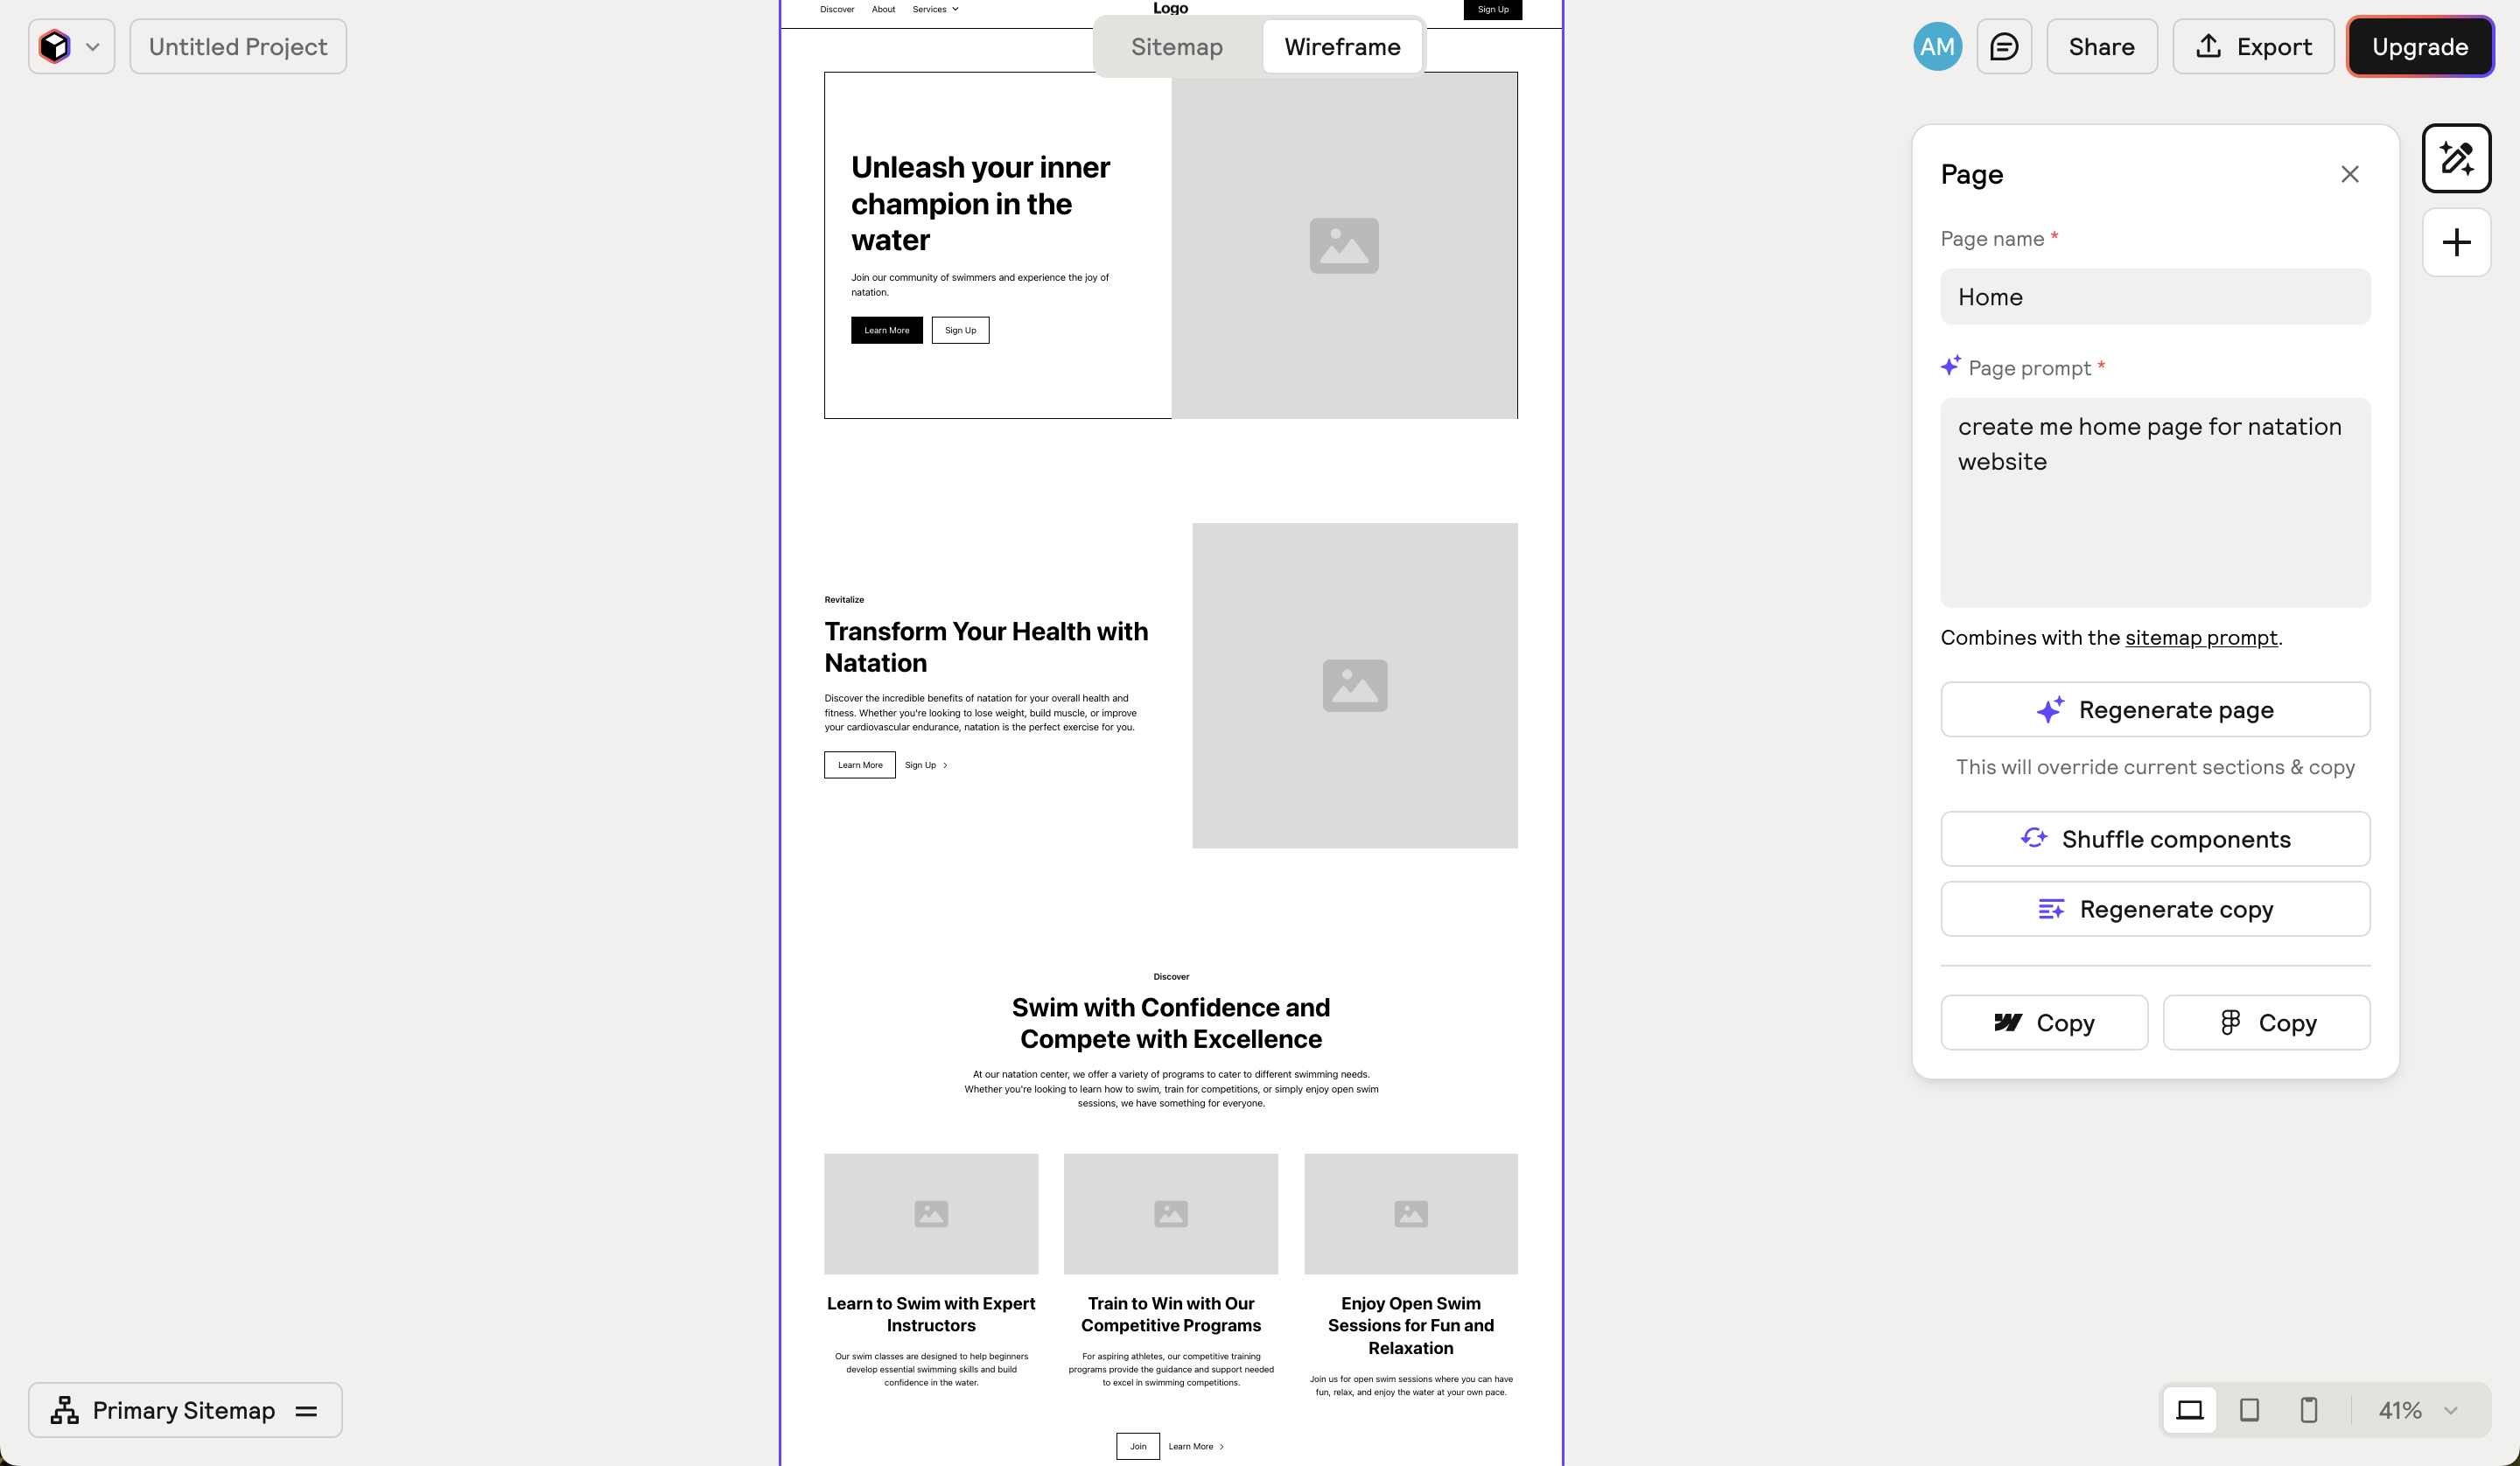
\includegraphics[width=0.8\textwidth]{Includes/Images/relume.png}
  \caption{Exemple de génération de site web sur la natation avec Relume}
  \label{fig: relume}
\end{figure} 

De plus, Relume est particulièrement efficace pour les sites classiques, comme les sites e-commerce, qui utilisent souvent des composants récurrents tels que des carrousels, des barres de navigation, des pieds de page, etc. La génération automatique de ces éléments permet de gagner un temps précieux tout en garantissant une structure cohérente et professionnelle. Relume offre également la possibilité de générer des contenus textuels en français, bien que ceux-ci soient souvent génériques.


Nous pouvons voir un exemple d'une génération de site web sur la natation avec Relume, nous pouvons voir la structure du site, les pages et les composants générés automatiquement (voir figure \ref{fig: relume}).
C'est idéal pour les projets simples, Relume se distingue par sa capacité à augmenter la productivité tout en simplifiant la gestion des projets web. Toutefois, pour des projets plus complexes nécessitant des designs et des contenus plus personnalisés, l’intervention humaine reste indispensable. 

\subsection{Webflow}
Webflow est une plateforme innovante de conception et de développement de sites web qui permet de créer des sites professionnels sans nécessiter de compétences en codage. Intégrant un éditeur visuel intuitif, Webflow permet de concevoir et de personnaliser des pages web à l'aide de fonctionnalités de glisser-déposer, tout en appliquant des styles CSS en temps réel. Les capacités avancées d'interactions et d'animations permettent de créer des expériences utilisateur engageantes, sans écrire de code complexe. De plus, Webflow offre des possibilités de low code, permettant aux développeurs d'ajouter des fonctionnalités personnalisées à travers des snippets de code et des intégrations avec d'autres outils, enrichissant ainsi l'expérience et les capacités du site. Webflow représente ainsi une solution complète et accessible alliant design esthétique et performance technique.

\subsection{DevLink}
DevLink constitue un outil de WebFlow qui facilite l'intégration des composants créés dans WebFlow à notre code (exclusivement React). Cette fonctionnalité permet d'exporter les composants créés dans WebFlow directement en code React via une simple ligne de commande. De surcroît, elle assure la synchronisation de nos composants dans notre code avec WebFlow. Ainsi, nous sommes en mesure d'importer les composants élaborés sur WebFlow dans notre code React, et de les mettre à jour automatiquement lorsque le designer effectue des modifications depuis WebFlow. 

\subsection{Contentful}
Contentful est une plateforme de gestion de contenu (CMS headless) conçue pour répondre aux besoins des développeurs. Avec son architecture flexible basée sur le cloud et son API robuste, Contentful offre une solution de gestion de contenu, les développeurs peuvent facilement intégrer Contentful à n'importe quelle technologie frontend grâce à ses API RESTful et GraphQL. Cela permet une séparation claire entre le backend et le frontend, offrant ainsi une plus grande liberté de conception et une expérience de développement plus fluide. De plus, Contentful prend en charge la collaboration en équipe avec des fonctionnalités telles que les environnements de développement, les workflows de contenu et la gestion des droits d'accès, ce qui en fait un outil incontournable pour créer des expériences web dynamiques et évolutives.

\section{Reflexion sur les difféntes possibilité d'interactions entre les outils}
Avec l'équipe nous avons réflechie sur les difféntes possiblités d'interactions.

\subsection{Possibilité n°1 - Basique}
\begin{figure}[h] 
  \centering
  
\includegraphics[width=1\textwidth]{Includes/Images/connection1.png}
  \caption{Schéma de la possibilité n°1 - Basique}
  \label{fig: Schéma de la possibilité n°1 - Basique}
\end{figure} 
La première option, la plus basique, consiste à rassembler simplement les outils (voir figure \ref{fig: Schéma de la possibilité n°1 - Basique}). Le but est de créer le site sur Relume, qui génère toute l'expérience utilisateur (UX), les wireframes, les composants et le texte. Ensuite, nous transférons tout ce que nous avons construit sur Webflow pour créer l'interface utilisateur (UI), styliser le site, ajouter des animations, etc. Enfin, avec DevLink, nous exportons tous nos composants pour les intégrer dans notre code React. Cependant, tout le texte et le contenu sont codés en dur. Si nous souhaitons modifier le texte ou les images, nous devons resynchroniser DevLink et reconstruire le site avec Next.js.

Cette méthode présente l'avantage de simplifier le processus initial de création et de design, mais elle impose des contraintes en termes de maintenance et de mises à jour de contenu. Pour chaque modification de texte ou d'image, il est nécessaire de passer par une étape de synchronisation et de reconstruction, ce qui peut être laborieux et chronophage.

\subsection{Possibilité n°2 - Avec un CMS}

Avec un CMS : L'objectif ici est de connecter Relume directement ou indirectement (via un webhook) à un CMS, afin que Relume prenne en compte le texte du CMS et l'enregistre à chaque génération. Cela permet de rendre le texte modifiable dynamiquement dans le CMS et de ne pas le perdre à chaque régénération des wireframes.

\begin{figure}[h] 
  \centering
  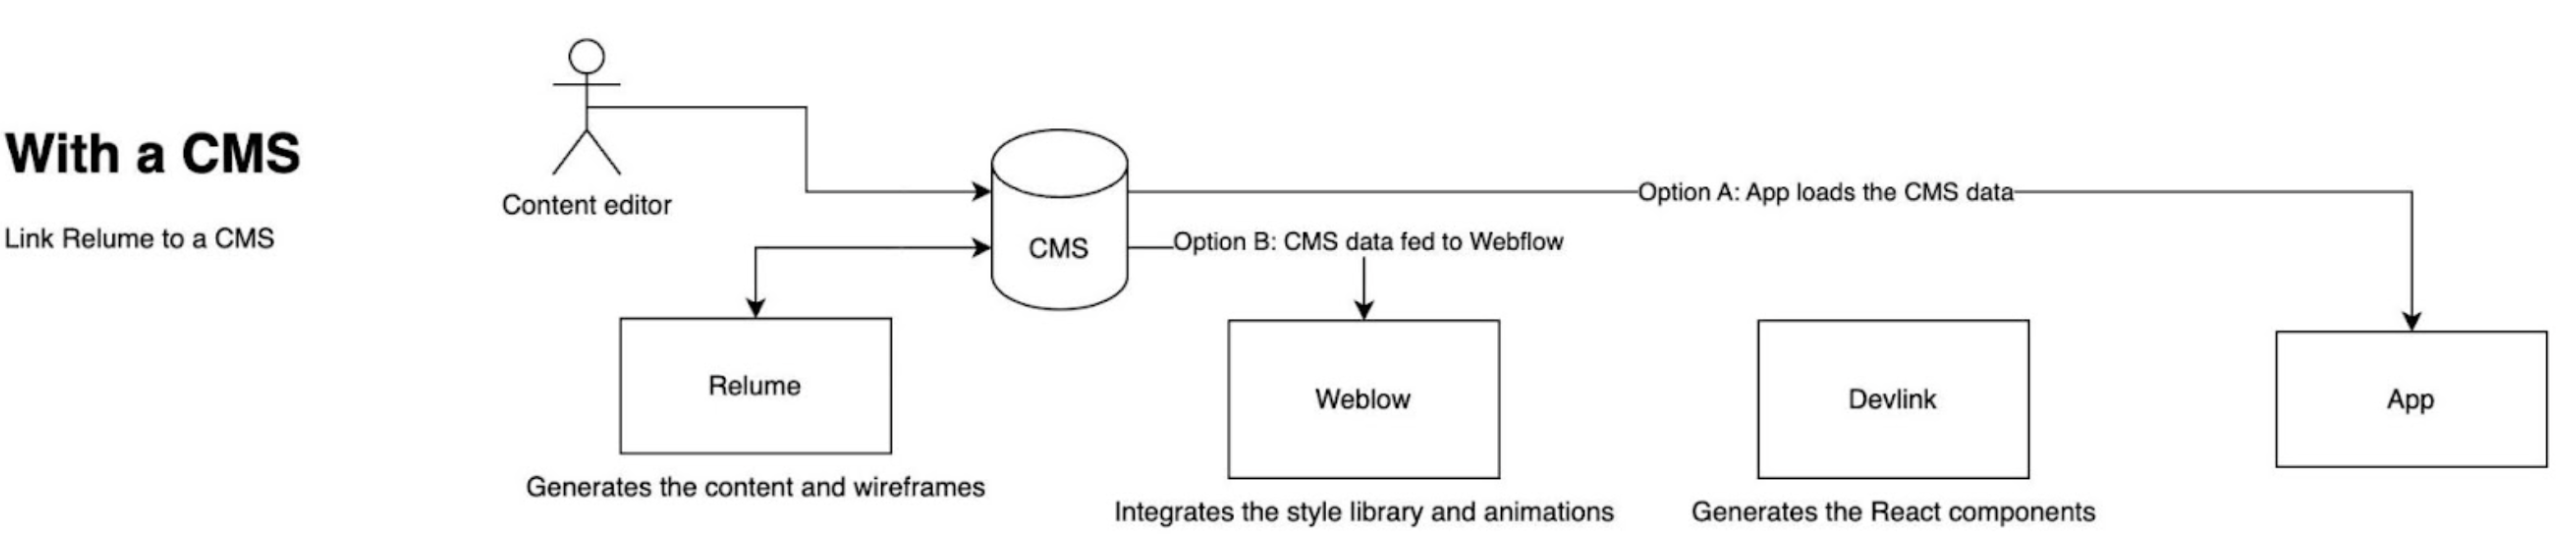
\includegraphics[width=1\textwidth]{Includes/Images/connection2.png}
  \caption{Possibilité n°2 - Avec un CMS, option A}
  \label{fig: Possibilité n°2 - Avec un CMS, option A}
\end{figure} 

Option A : Récupérer les données de la base de code React et transmettre ces données en tant que props.

\begin{figure}[h] 
  \centering
  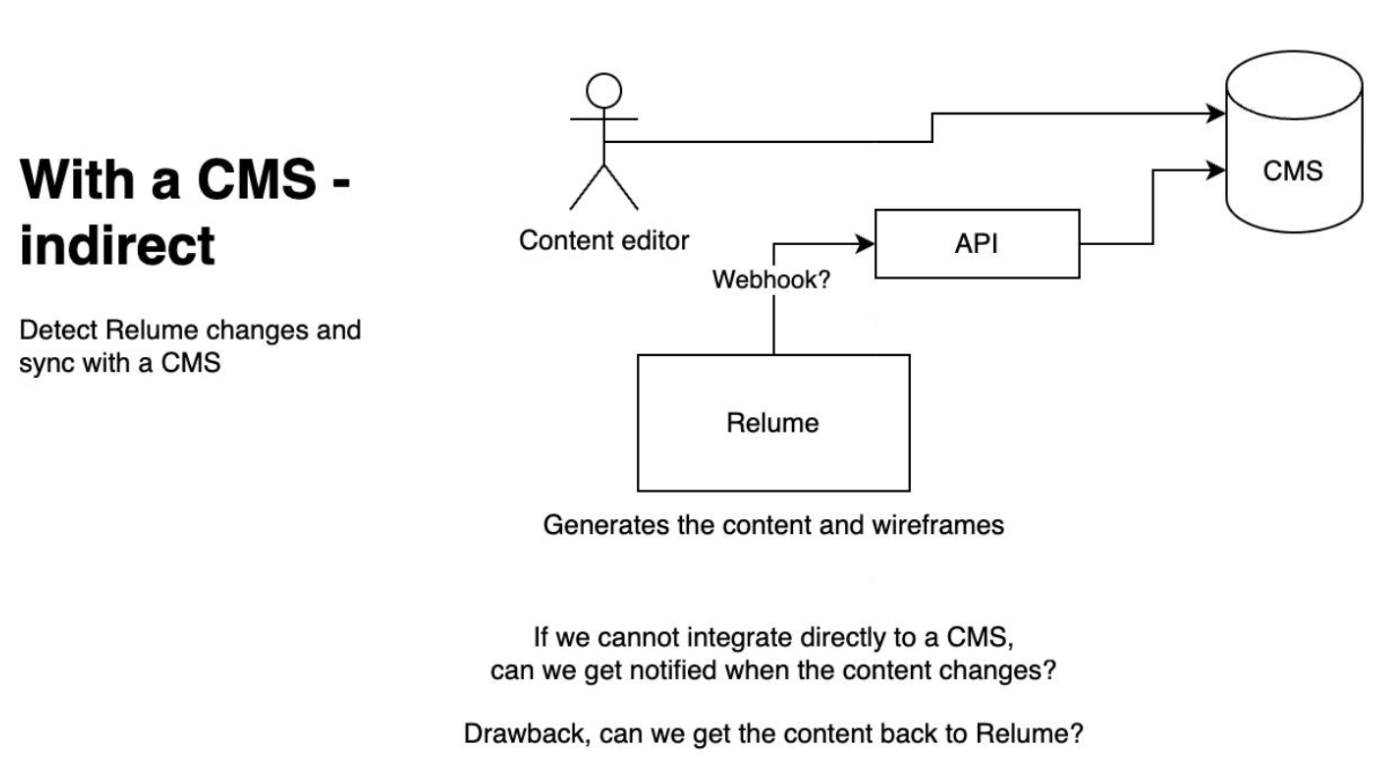
\includegraphics[width=1\textwidth]{Includes/Images/connection3.png}
  \caption{Possibilité n°2 - Avec un CMS, option B}
  \label{fig: Possibilité n°2 - Avec un CMS, option B}
\end{figure} 

Option B : Récupérer le texte et les données du CMS dans Webflow pour les exporter avec des données dynamiques. Cependant, cette méthode nécessiterait une nouvelle exportation à chaque fois qu'il y a un changement dans les informations.

Cette approche offre la flexibilité de modifier le contenu directement dans le CMS sans avoir à resynchroniser et reconstruire l'ensemble du site. Elle permet également de maintenir le contenu à jour plus facilement, bien que l'option B puisse impliquer des opérations supplémentaires lors de chaque modification des informations.
% DEVELOPMENT CONTEXT
% \include{Includes/contexteDeveloppement}
\EmptyPage
\chapter{Bilan et critique des résultats}

\section{Comparaison avec le cahier des charges}

Les objectifs du cahier des charges ont été partiellement atteints :

\begin{itemize}
    \item Test des outils et services : réussi.
    \item Étude des interactions : réussie, mais avec des limitations.
    \item Développement du prototype : réussi.
    \item Évaluation de la solution : réussie, avec des limitations identifiées.
\end{itemize}

\section{Difficultés rencontrées}

Les principales difficultés incluent le manque de documentation pour Relume et les limitations de DevLink avec certains composants Webflow.

\section{Enseignements tirés}

Il est crucial de choisir des outils avec une documentation complète et un support technique robuste. Une analyse approfondie de la compatibilité des outils dès le départ est également essentielle. Adopter une approche itérative permet de s'adapter aux défis rencontrés et d'améliorer progressivement la solution.


% creationInterface
% \include{Includes/creationInterface}
\EmptyPage
% CONCLUSIONS
\chapter{Conclusion}
Mon travail au sein de l'entreprise DEPT a été axé sur le développement d'une solution innovante visant à optimiser le processus de création d'interfaces utilisateur dynamiques. Ce projet a abouti à la création d'un prototype fonctionnel intégrant divers outils et technologies modernes.

Sur le plan de ma contribution à l'entreprise, j'ai réussi à créer une solution qui simplifie et accélère le processus de création, tout en améliorant la collaboration entre les différents métiers impliqués. Cette solution ouvre également la voie à de futures améliorations et évolutions, notamment en termes de tests et de déploiement à grande échelle. Les perspectives pour cette solution incluent son intégration dans les processus de développement de l'entreprise, ainsi que son éventuelle adoption par d'autres équipes ou projets.

Sur le plan personnel, ce stage m'a apporté une multitude d'enseignements et d'expériences enrichissantes. J'ai pu apprendre de nouvelles compétences techniques, notamment en matière de développement front-end et d'intégration avec des CMS headless. De plus, j'ai pu bénéficier d'un encadrement précieux de la part de M. Marc Raffalli, qui m'a guidé à travers les défis techniques et m'a permis de mieux comprendre l'architecture logicielle. Enfin, ce stage m'a offert l'opportunité de découvrir le fonctionnement d'une entreprise internationale, d'explorer de nouvelles méthodes de travail et de renforcer ma passion pour le développement web.

En somme, ce stage chez DEPT a été une expérience extrêmement enrichissante à la fois sur le plan professionnel et personnel. Il m'a permis de contribuer activement à un projet concret tout en développant mes compétences et en élargissant mes horizons dans le domaine du développement web.
\EmptyPage
% TABLES OF FIGURES
\listoffigures
\chapter*{Webographie}
\begin{enumerate}
  \item \href{https://www.youtube.com/watch?v=6Qw06niEs0I&t}{Documentation de Javascript} \label{doc:javascript}
  \item \href{https://react.dev/}{Documentation de React} \label{doc:react}
  \item \href{https://nextjs.org/docs}{Documentation de Next.js} \label{doc:nextjs}
  \item \href{https://www.contentful.com/developers/docs/}{Documentation ContentFul} \label{doc:contentful}
  \item \href{https://developers.webflow.com/}{Documentation de Webflow} \label{doc:webflow}
  \item  \href{https://www.relume.io/}{Relume} \label{doc:relume}
  \item \href{https://www.youtube.com/@Relume_io}{Chaîne Youtube de Relume} \label{doc:yb-relume} 
  \item \href{https://docs.developers.webflow.com/data/docs/devlink-documentation-and-usage-guide}{Documentation de DevLink} \label{doc:devlink}
  \item \href{https://www.youtube.com/watch?v=6Qw06niEs0I&t}{Connecter Relume avec un CMS} \label{doc:relume-cms}
  \item \href{https://www.youtube.com/watch?v=HMsrFzoZYr0}{Connecter Webflow avec un CMS headless externe} \label{doc:webflow-cms}
\end{enumerate}

\EmptyPage
\end{document}

